\documentclass{template/socthesis}

\usepackage[czech]{babel}
\usepackage[T1]{fontenc} % evropské uvozovky
\usepackage{csquotes}
\usepackage{xpatch}
\usepackage[author=,status=draft]{fixme} % vkládání poznámek  
% dva módy (status): draft (poznámky se zobrazují v PDF) / final (poznámky se nezobrazují v PDF)

\usepackage{subcaption}
\usepackage[backend=bibtex,bibstyle=numeric,sorting=none,date=long,dateabbrev=false,texencoding=utf8,bibencoding=utf8,style=iso-numeric]{biblatex}
\usepackage{amsmath}
\usepackage{enumitem}

\addbibresource{text.bib}

\titlecz{SDK pro výuku programování na IoT stavebnici}
\titleen{SDK for educational IoT kit}
\author{Tomáš Rohlínek}
\field{18} % Obory SOČ: 1 - 18 (http://www.soc.cz/obory-soc/)
\school{Střední průmyslová škola a Vyšší odborná škola Brno, Sokolská, příspěvková organizace}
\mentor{Vojtěch Boček}
\mentorstatement{Vojtěchu Bočkovi}

% Změňte, pokud se liší
%\region{Jihomoravský}
% \placefooter{Brno 2017}

\begin{document}

\maketitle

\makecopyrightstatement{V~Drásově}

\makethanks{Děkuji svému školiteli Vojtěchu Bočkovi}
\fxfatal{Dopsat poděkování}

\pagestyle{empty}

\section*{Anotace}
Cílem této práce je vytvořit SDK pro práci a výuku na IoT stavebnici BlackBox postavené na platformě ESP32. \fxfatal{odkaz}

\subsection*{Klíčová slova}
BlackBox; IoT; \fxnote{další buzz slovíčka}

\vspace{20mm}

\section*{Annotation}
\fxfatal{překlad}

\subsection*{Keywords}
\fxfatal{překlad}

\newpage
\pagestyle{plain}

\tableofcontents % vysází obsah

%%% Začátek práce
\setcounter{figure}{0}
\setcounter{table}{0}
\newpage

%%% Úvod
\chapter*{Úvod}

V létě roku 2019 jsem vedl robotický tábor a potřeboval jsem narychlo nachystat výrobek, který bychom mohli s účastníky programovat.
Vznikl tak první elektronický trezor později pojmenovaný BlackBox.

Od té doby prošel hardware několika verzemi, od kupky Arduino modulů po komplexní desku.
Jakkoliv dobrý hardware však v dnešní době není nic bez softwaru, který by ho řídil, proto vznikla tato práce.
Jejím cílem je napsat SDK pro desku BlackBox a to pro tři skupiny lidí, organizátory outdoorových her, učitele programování a běžné robotiky.
Nutno podotknout, že se práce nezabývá vytvořením hardwarové části, to je náplní samostatné práce\cite{BlackBox_hardware}.

% \fxnote{"zařízení" není to nejlepší slovo}
% The purpose of this work is to create a~"device" that can be used as both educational development kit and tool for creating complex outdoor games with minimal/automated setup and maximum reusability

% \fxnote{možná použít historii jako odstavec? (jak to vše začalo)}

\newpage
\chapter{Krátké shrnutí možností hardware}
Můj software je psaný pro stavebnici BlackBox, která byla vytvořená Tomášem Vavrincem. 
Aktuální verze hardware (v1.1) obsahuje následující funkční bloky:

\begin{figure}
    \begin{small}
        \begin{center}
            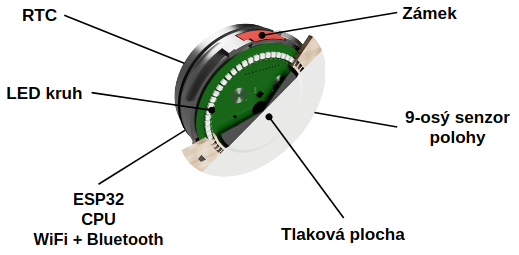
\includegraphics[width=0.95\textwidth]{img/hardware.png}
        \end{center}
        \caption{Hardware}
        \label{fig:hardware}
    \end{small}
\end{figure}

\begin{itemize}[noitemsep]
    \item Hlavní řídící modul
        \begin{itemize}[noitemsep]
            \item ESP32 včetně Wi-fi a bluetooth
            \item Real Time Clock
        \end{itemize}
    \item Uživatelské rozhraní
          \begin{itemize}[noitemsep]
              \item Touchpad
              \item LED kruh
          \end{itemize}
    \item Zámek
        \begin{itemize}[noitemsep]
            \item Motor
            \item Enkodér
            \item IR přijímač
            \item IR vysílač
            \item Zámek sériové linky
        \end{itemize}
    \item Senzory prostředí
          \begin{itemize}[noitemsep]
              \item Magnetometr
              \item Akcelerometr
              \item Gyroskop
              \item Barometr
          \end{itemize}
\end{itemize}

\newpage
\section{Hlavní řídící modul}
Hlavní řídící modul slouží jako výpočetní a~řídící centrum celé desky.

\subsection{ESP32}
BlackBox používá ESP32-WROVER jako svůj procesor.
Základní informace:
\begin{itemize}
    \item Dual core
    \item 240~MHz
    \item 4MB flash
    \item 8MB PSRAM
    \item WiFi, Bluetooth
\end{itemize}

\subsection{Real Time Clock}
Kvůli snížení spotřeby energie bylo implementováno několik mechanismů
Jeden z~těchto mechanismů je i~vypínání všech nepotřebných periferií a~uspání ESP32.V~takovém případě ale není možné uchovat aktuální čas, proto byl na BlackBox přidán modul RTC, ten je napájen přímo z~baterií a~není tak závislý na zbytku BlackBoxu.

\section{Uživatelské rozhraní}

\subsection{Touchpad}
Touchpad je postavený na čipu LDC1614 a jeho alternativách.\footnote{Použitelné jsou pouze alternativy se 4~kanály t.j.~ty, co mají tvar názvu LDCXX14}
Pro měření stisku se využívá deformace kovové destičky a~indukčního měření její vzdálenosti od 4~plošných cívek.
\fxnote{Tady se dá potenciálně napsat spousta věcí :D}

\subsection{LED kruh}
Kruh sestává z~60~adresovatelných RGB LED diod typu WS2812B.

\section{Zámek}

\subsection{Motor a~Encodér}
Zamykací mechanismus je sestaven tak, aby šel BlackBox zasunout do zad trezoru i~v zamčeném stavu, obejde se tedy bez kontroly toho, jestli je při zamykání zasunutý nebo ne.

\subsection{IR komunikace}
IR komunikace je zde obsažená hlavně kvůli synchronizaci se zády trezoru, přesněji k~identifikaci, do kterých zad je BlackBox zasunut.
Tato identifikace by se potenciálně dala dělat pomocí senzorů prostředí, ale za účelem jednoduchosti a~redundance byla zvolena tato možnost.

\subsection{Zámek sériové linky}
Tento mechanismus byl navrhnut za účelem ochrany BlackBox proti neautorizovanému přepsání softwaru.

\section{Senzory prostředí}

\subsection{Senzory polohy}
Tato sada senzorů (akcelerometr, gyroskop, magnetometr) je na různých verzích desky realizována různým způsobem, na verzi 1.0~je realizována jedním čipem obsahujícím všechny tři senzory, ale na verzi 1.1~je realizována pomocí dvou čipů (akcelerometr + gyroskop a~magnetometr)\footnote{Verze 1.1~je zpětně kompatibilní, takže se na ni dá osadit i~čip z~verze 1.0, toho je však v~době psaní této práce nedostatek a~proto byl nahrazen na verzi 1.1 dvěma běžnějšími čipy.}.
Knihovna však musí podporovat všechny možnosti.
Tyto senzory zjišťují natočení BlackBoxu v~prostoru v~9ti osách.
Do budoucna se chystá rozšíření o~GPS senzor.

\subsection{Barometr}
Barometr zde slouží hlavně k hrubému měření výšky, na které se BlackBox nachází.
Případně se také dá použít jako primitivní způsob předpovědi počasí.

\chapter{Architektura}

Projekt je rozdělený na tři vrstvy:

\begin{enumerate}
    \item Řídící prvky hardwaru

    Jednotlivé knihovny pro práci s hardwarem teoreticky použitelné mimo prostředí BlackBox

    \item Manager hardware prvků
    
    Třída určená pro jednoduchou práci se všemi prvky hardware naráz, aniž by docházelo ke kolizím

    \item Game engine
    
    \fxnote{popis co to má být}
\end{enumerate}

\newpage
\printbibliography[title=Literatura]
\addcontentsline{toc}{section}{Literatura}

\listoffigures
\addcontentsline{toc}{section}{Seznam obrázků}

\listoftables
\addcontentsline{toc}{section}{Seznam tabulek}

\listoflistedequation
\addcontentsline{toc}{section}{Seznam rovnic}

\end{document}
